\section{INTRODUCTION}


\subsection{Adversarial Attacks}
Adversarial attacks are those malicious attacks on the data which may seem okay to the human eye but causes misclassification in a machine-learning pipeline. These attacks are often made in the form of specially designed “noise,” which causes misclassification.
An Adversarial Attack is a technique to find a perturbation that changes the prediction of a machine learning model.
Adversarial attacks are crafted to find the vulnerabilities in the Machine Learning (ML) models which later can be used to improve the robustness of a neural network or ML model. The following Figure shows the generation of an Adversarial example by adding a small amount of noise in it.\\

\begin{figure}[!hbt]
    \centering
    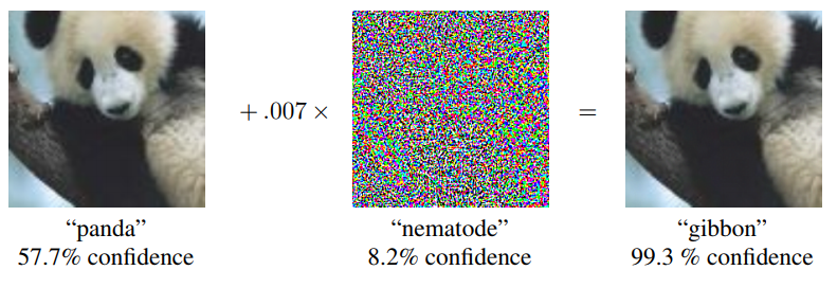
\includegraphics[scale=0.6]{img/Picture2.png}
    \caption{An Adversarial Example}
    \label{fig:Figure1}
\end{figure}

Some example Applications of adversarial attacks are:
\begin{itemize}
  \item Fooling an Automated Vehicle System.
  \item Hacking a Face Recognition System (FRS) in public camera surveillance (CCTV).
\end{itemize}

\begin{figure}[!hbt]
    \centering
    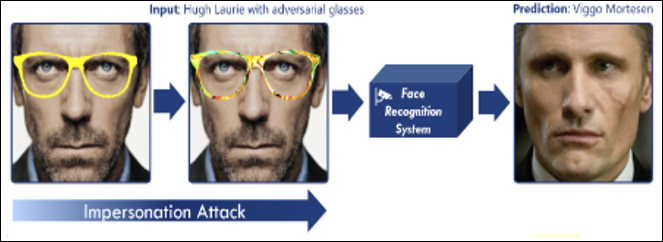
\includegraphics[scale=0.7]{img/Picture1.png}
    \caption{Hacking a Face Recognition System (FRS)}
    \label{fig:Figure1}
\end{figure}



\subsection{Types of Adversarial Attacks}
Adversarial attacks typically target neural networks, such as convolutional neural networks (CNNs) used for image classification or recurrent neural networks (RNNs) used for natural language processing. \\[1cm]
The key characteristics of adversarial attacks include:

\textbf{Perturbation:} Adversarial attacks involve introducing small, carefully crafted perturbations to the input data. These perturbations are typically imperceptible to human observers but can have a significant impact on the model's output.

\textbf{Transferability:} Adversarial examples generated for one model often work on other models trained on similar tasks. This means that an attacker can create a single adversarial example that can fool multiple different models.

There are different types of adversarial attacks, including:
\begin{itemize}
    \item \textbf{White-box attacks:} The attacker has complete knowledge of the target model, including its architecture and parameters, and can craft adversarial examples accordingly.

    \item \textbf{Black-box attacks:} The attacker has limited or no knowledge of the target model but can still generate adversarial examples by probing the model's responses and using them to craft attacks.

    \item \textbf{Transfer attacks:} Adversarial examples crafted for one model are used to attack a different model, even when the attacker has no knowledge of the target model's internals.

    \item \textbf{Non-targeted attacks:} These aim to cause misclassification without specifying the target class.

    \item \textbf{Targeted attacks:} These aim to cause the model to classify the input as a specific, predefined class.

\end{itemize}
 The following Table shows the key characteristics of White-Box and Black-Box attack techniques:


\begin{table}[H]
\centering
\begin{tabular}{|c|c|}
\hline
\textbf{White-Box Attack} & \textbf{Black-Box Attack}\\
\hline
Network architecture & Quering the model on input \\
\hline 
Input, output & Observing the labels \\
\hline
Training Data &   \\
\hline
Weights, and hyperparameters &   \\
 \hline
\end{tabular}
\caption{Adversary Knowledge in various Adversarial Attack Techniques}
\label{tab:Table1}
\end{table}


\section{LITERATURE REVIEW}

\textbf{Intriguing Properties of Neural Networks}\\
Szegedy et al. [1] discovered that many machine learning classification models misclassify examples that are only slightly different from correctly classified examples drawn from the data distribution. They also discovered that various models with different architectures when trained on different subsets of the training data misclassify the same adversarial example. These discoveries show that there is a blind spot in our training algorithm where the adversarial examples are coming from.

\textbf{Explaining and harnessing adversarial examples}\\
Goodfellow et al. [2] give the cause of adversarial examples. They made the observation that the linear behavior of deep neural networks in high-dimensional spaces is sufficient to cause adversarial examples. Non-linearity helps resist adversarial perturbation but such networks are not easy to train and hence nonlinear models such as sigmoid networks are carefully tuned to spend most of their time in the non-saturating, more linear regime. This linear view of adversarial examples suggests a fast way of generating them which is referred to as the Fast Gradient Sign Method (FGSM).

\textbf{Black box adversarial attacks with bandit and priors}\\
Adversarial examples are slightly perturbed inputs designed to fool the network prediction. Such vulnerabilities give methods to form attacks (adversarial attacks) which turn out to be very effective i.e. a small number of gradient steps can construct an adversarial perturbation. A significant shortcoming of such attacks is that in white-box attack model we need access to the gradient of the classification loss of the attacked network but in a real-world scenario expecting this kind of complete access is not realistic. An adversary can only get response to the queries passed to a classification model and which gives a black-box attack model [4]. The gradient estimation problem is the central problem in the context of query-efficient black-box attacks. The paper discusses the black-box attacks and the gradient estimation problem. It exploits the prior knowledge about the availability of gradients to make a black-box attack query-efficient.

\textbf{Adversarial Attacks on Black Box Video Classifiers: Leveraging the Power of Geometric Transformations}\\
In black-box attack settings, effective gradients are estimated by searching for directions that maximize the probability of the victim model misclassifying the crafted inputs [6]. The paper talks about adversarial attack on video classification models which is query-efficient. To make an attack query-efficient it reduces the search space by defining this space with a small set of parameters which describe gradients in the temporal dimension. The main contribution of the paper is in reducing the dimensions of the search space for effective gradient calculation by making use of a sequence of geometric transformations.



\subsection{Literature Review: Summary}
\begin{itemize}
  \item \textbf{Balance:} There is no foolproof defense against all possible attacks. Adversarial attacks and defenses are often in a constant parallel race. 

  \item \textbf{Trade-offs:} Adversarial defenses often come with trade-offs, such as increased computational cost during training and inference, potential changes in model performance on clean data, and the risk of overfitting to the specific adversarial examples used during training.

  \item \textbf{Real-world use case:} In some cases, the cost and effort required to develop strong adversarial defenses may outweigh the potential risks of attacks. In other cases, security and robustness are critical, and strong defenses are necessary.


\end{itemize}

\section{SOTA ADVERSARIAL ATTACK TECHNIQUE: STYLEFOOL}
% \subsection{StyleFool}

\subsection{Abstract}
Video adversarial attacks are a type of cyberattack that can fool video classification systems into making incorrect predictions. These attacks can have serious consequences, such as enabling unauthorized access to secure areas or preventing the detection of criminal activity.
StyleFool is a new black-box video adversarial attack that uses style transfer to create imperceptible adversarial videos. StyleFool is more effective than existing attacks because it uses a gradient-free optimization method that does not require a large number of queries. Additionally, StyleFool is more robust to defenses such as denoising and adversarial training.
\begin{itemize}
    \item[-]\textbf{Key findings:}
    \item StyleFool outperforms other adversarial attacks in terms of both the number of queries and the robustness against existing defenses.
    \item 50\% of the stylized videos in untargeted attacks do not need any queries since they can already fool the video classification model.
    \item Adversarial samples of StyleFool look imperceptible to human eyes.
\end{itemize}

\subsection{Threat Model}

\begin{itemize}
    \item \textbf{Adversary's goals: } Given a DNN, it takes a video x from a video set X as input. The model outputs a K-class prediction label y, $y \in Y$. Adversary's goal is to find $x_{adv} $ such that, 
    \begin{figure}[!hbt]
    \centering
    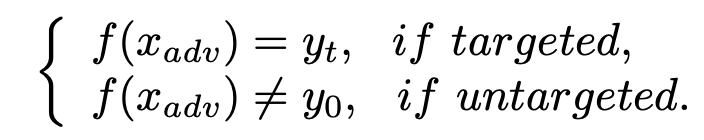
\includegraphics[scale=0.4]{img/goals.png}
    % \caption{An Adversarial Example}
    % \label{fig:Figure1}
    \end{figure}
    \item \textbf{Adversary's capabilities: } The adversary is capable of crafting perturbations and superimposing them on given videos in the offline setting. To establish a video frame set from which the style images could be selected, the adversary use publically available dataset.
    \item \textbf{Adversary's knowledge: } Adopted  query limited partial information setting. That is, put an upper limit bound on attacker's queries and access to only top-1 label y with its confidence score, based on confidence score.
\end{itemize}

\subsection{Design and Algorithm: StyleFool}
The framework of StyleFool is depicted in Figure 3. At first, according to the style selection criteria, the best style is selected for style transfer. Then, by considering content, style, total variance, and temporal loss terms, the clean video is transferred into the selected style. Finally, a black-box adversarial attack is conducted to consolidate perturbations that can fool the target model.
\begin{figure}[!hbt]
    \centering
    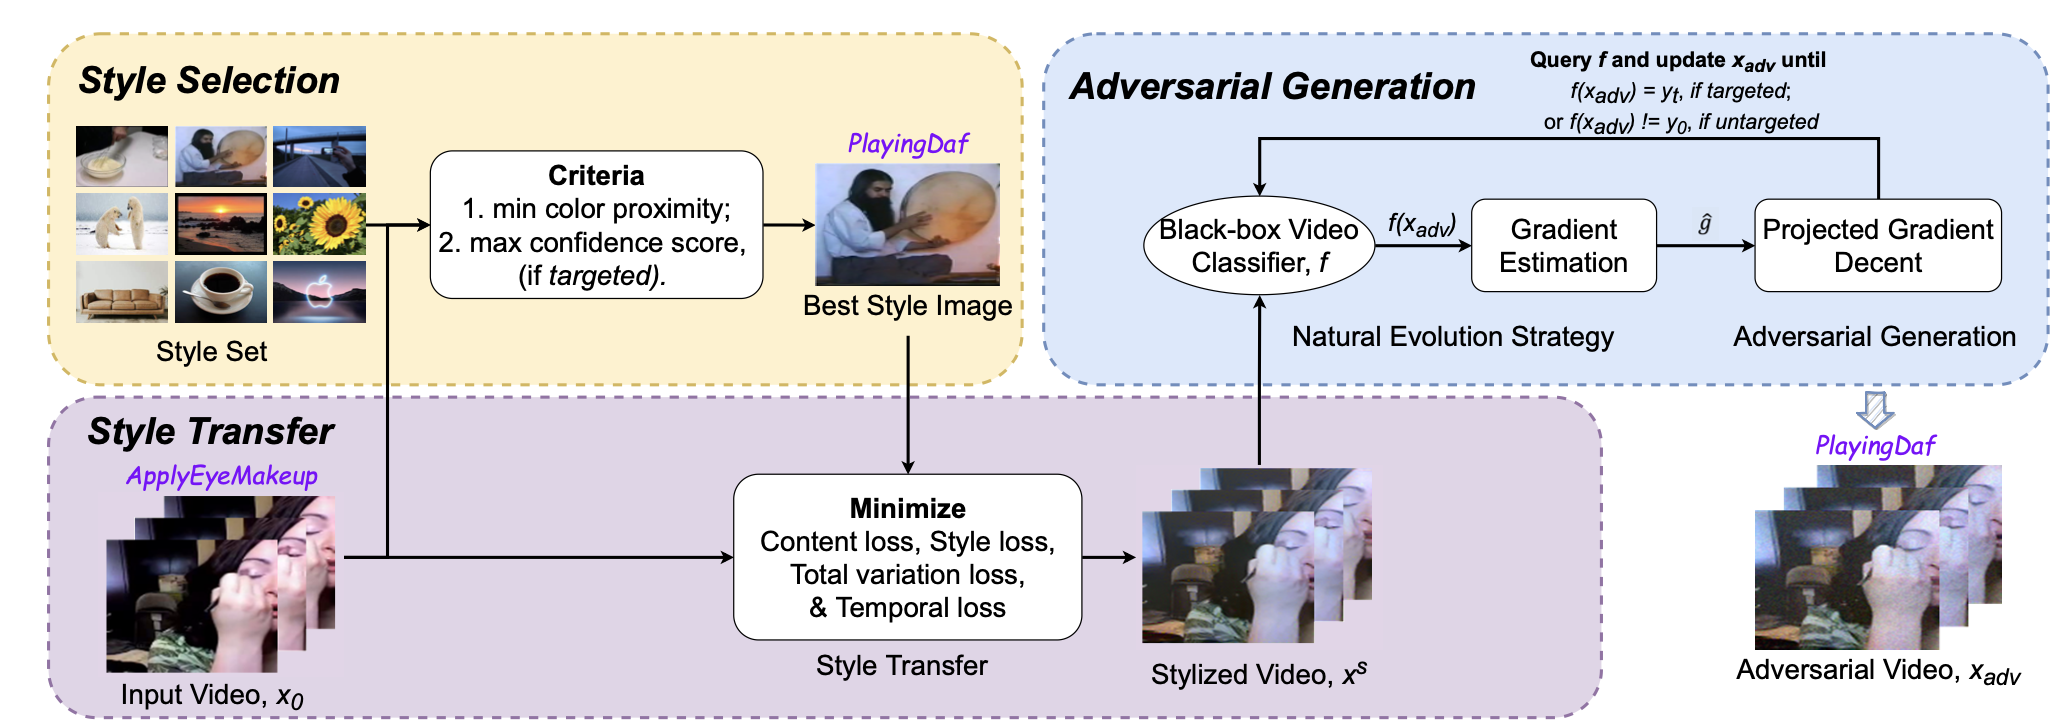
\includegraphics[scale=0.28]{img/framework.png}
    \caption{Framework}
    \label{fig:Figure3}
\end{figure}

\subsubsection{Style Selection}
Style selection is a crucial step in StyleFool to ensure the stylized videos are indistinguishable from the original videos, and to help initialize the stylized video in the vicinity of the decision boundary. 
To achieve indistinguishability, StyleFool proposes two style selection approaches:
\begin{itemize}
    \item \textbf{Color Proximity:} This approach selects style images that are visually similar to the original videos. This helps to preserve the naturalness of the stylized videos.
    \item \textbf{Stylized Boundary Search:} This approach selects style images that are likely to move the videos closer to the decision boundary of the target class. This helps to reduce the number of queries required to craft adversarial videos.
    \begin{figure}[!hbt]
    \centering
    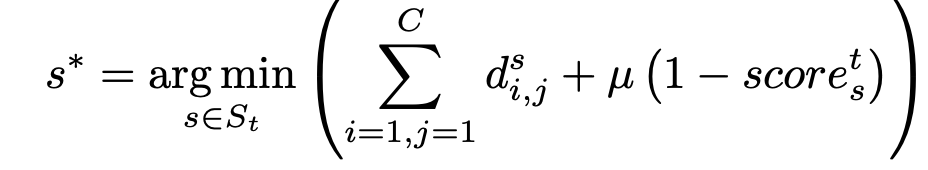
\includegraphics[scale=0.4]{img/styleSelection.png}
    \caption{Principle of style image selection for targeted attack}
    % \label{fig:Figure3} 
    \end{figure}
\end{itemize}

\subsubsection{Style Transfer}
StyleFool's style transfer stage uses a total loss function that includes content loss, style loss, total variation regularizer loss, and temporal loss.
\begin{itemize}
    \item Content loss encourages the stylized video to be similar to the original video in terms of its high-level representations.
    \item Style loss encourages the stylized video to be similar to the style image in terms of its feature distributions.
    \item Total variation regularizer loss eliminates noise or shadow and improves the smoothness of each stylized image.
    \item Temporal loss improves the consistency between two consecutive frames.
\end{itemize}
$ L_{total} = \sum (a.L_{content}(x_i, x_{i+1}) + b.L_{style}(x_{i}^{s}, s) + c.L_{tv}(x_{i}^{s})) + d.\sum L_{temporal}(x_{i}^{s}, x_{i+1}^{s})$

\subsubsection{Adversarial Sample Generation}
StyleFool is a black-box video adversarial attack that uses style transfer to create imperceptible adversarial videos. It achieves this by estimating the gradients of the loss function using Natural Evolution Strategy (NES). NES is a gradient estimation method that is particularly well-suited for black-box attacks because it does not require access to the model structure or parameters. StyleFool uses antithetic sampling to reduce the variance of the gradient estimates. This makes the attack more efficient and less likely to get stuck in local minima. For targeted attacks, StyleFool begins with an instance from the target class and optimizes it using Projected Gradient Decent (PGD). This ensures that the adversarial video is still classified as the target class. For untargeted attacks, StyleFool directly takes the stylized video as the initial value of $x_{adv}$. This makes the attack even more efficient.

\begin{table}[H]
\centering
\begin{tabular}{ |c|c|  }
\hline
 Gradient estimation method & Natural Evolution Strategy (NES)  \\ 
 \hline
 Variance reduction technique & Antithetic sampling  \\  
 \hline
 Targeted attack optimization method & Projected Gradient Decent (PGD) \\
 \hline
 Untargeted attack optimization method & Direct use of stylized video \\
 \hline
\end{tabular}
\caption{Feature and their Description}
\label{tab:Table1}
\end{table}


\subsubsection{Algorithm}

\begin{figure}[!hbt]
    \centering
    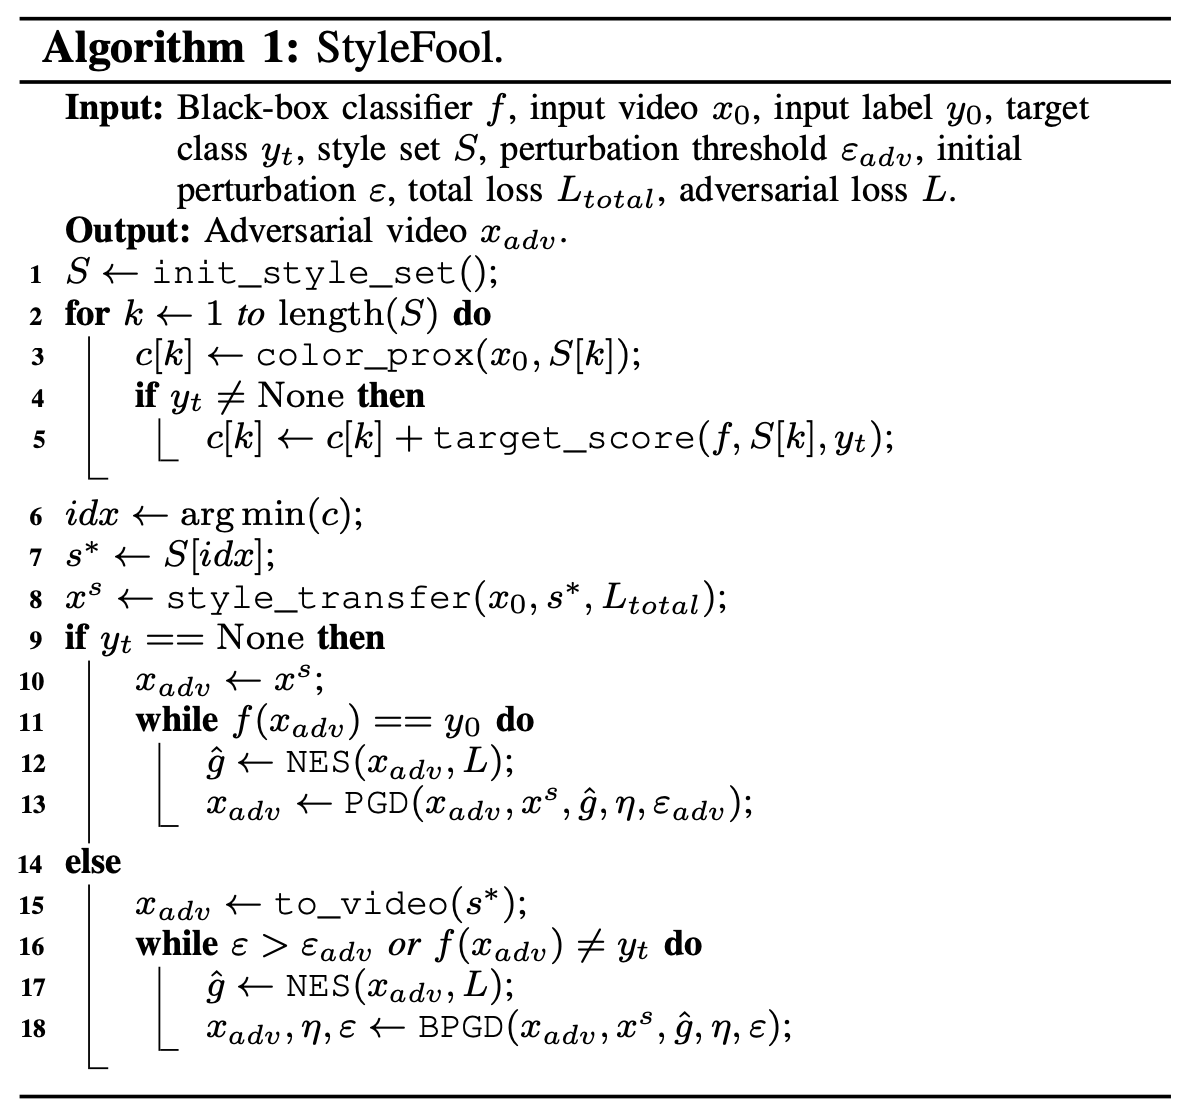
\includegraphics[scale=0.5]{img/algorithm.png}
    \caption{StyleFool Algorithm}
    \label{fig:Figure5}
\end{figure}

\subsection{Reproducing results of SOTA}

For reproduction of results, StyleFool was evaluated on UCF101 dataset with targeted attack on C3D. C3D learns both spatial and tem- poral features of input videos using 3D convolution. UCF-101 is an action recognition dataset collected from YouTube, containing 13,320 video samples with 101 action classes, e.g., archery, haircut, and punch.

Metrics defined during evaluation are as follows:
\begin{itemize}
    \item[-] \textbf{Attack Success Rate (ASR):} the ratio of adversarial videos that successfully mislead the classifier.
    \item[-] \textbf{Minimal Queries (minQ), Maximal Queries (maxQ), and Average Queries (AQ):} the minimal, maximal, and average numbers of queries to succeed in an attack. For fair comparison, in StyleFool, the number of queries during style selection is also counted, although this proportion is quite small.
    \item[-] \textbf{Indistinguishability:} the naturalness and realness of videos. 
\end{itemize}

\textbf{Experimental Results: }
Evaluation set (UCF-101), Hardware used: RTX3070i

\begin{table}[H]
\centering
\begin{tabular}{|c|c|c|c|c|}
\hline
\textbf{Type of attack} & \textbf{ASR} & \textbf{minQ} & \textbf{maxQ} & \textbf{AvgQ}\\
\hline
Untargeted attack & 100 & 1 & 19,031 & 3,811 \\
\hline 
Targeted attack & 100 & 1284 & 248,131 & 65,066 \\
 \hline
\end{tabular}
\caption{Observed metrics during reproduction}
\label{tab:Table1}
\end{table}

\begin{table}[H]
\centering
\begin{tabular}{|c|c|c|}
\hline
\textbf{Type of attack} & \textbf{Preparation per image (sec)} & \textbf{Attack time cost (min)} \\
\hline
Untargeted attack & 0.42 & 1  \\
\hline 
Targeted attack & 0.42 & 10 \\
 \hline
\end{tabular}
\caption{Time costs}
\label{tab:Table1}
\end{table}

\subsection{Limitations}
StyleFool is a powerful and effective black-box video adversarial attack, but it does have some limitations.

\begin{itemize}
    \item \textbf{Computational complexity:} The style selection stage of StyleFool is computationally expensive. This is because it requires generating styles, calculating color themes, and calculating target class confidence. The complexity of this stage is O(class x N x Dim), where class is the number of classes in the target dataset, N is the number of videos in the target dataset, and Dim is the dimensionality of the feature space.
    \item \textbf{Imperceptibility of unrestricted perturbations:} Unrestricted perturbations are not always imperceptible to human eyes. This is because they can cause noticeable changes to the video's appearance.
\end{itemize}

\section {PROPOSAL: NOVELTY \& FEASIBILITY}

\subsection{Noval Idea: Proposal}
In the context of adversarial attacks, we introduce a novel method designed to address inherent limitations. This approach is aimed at crafting adversarial videos while considering various aspects such as black-box classifier f, input video $x_0$, input label $y_0$, target class $y_t$, perturbation threshold $\epsilon_{adv}$, initial perturbation $\epsilon$, total loss $L_{total}$, adversarial loss L, and structured noise \textit{N}.

The primary objective is to generate an adversarial video, denoted as $x_{adv}$, with the following algorithm:
\begin{itemize}
    \item[1.] Begin with the input video $x_0$ and apply structured noise \textit{N}, resulting in $x_s$, a video where structured noise has been introduced in place of the traditional style set. This step is crucial for preserving the content of the original video while introducing subtle perturbations.
    \item[2.] If the target class $y_t$ is not specified ($y_t == None$), we perform the following steps:
    \begin{itemize}
        \item[i.] Set $x_{adv}$ initially as $x_{s}$.
        \item[ii.] Apply Projected Gradient Descent (PGD) to iteratively update $x_{adv}$. The process continues until the perturbed video satisfies two conditions: a) it does not match the original label $y_0$, and b) the perturbation remains within the specified threshold $\epsilon_{adv}$. 
    \end{itemize}
    \item[3.] If a target class $y_t$ is specified, we proceed with the following steps:
    \begin{itemize}
        \item[i.] Set $x_{adv}$ initially as $x_s$.
        \item[ii.] Apply Biased Projected Gradient Descent (BPGD) to iteratively update $x_{adv}$. The process continues until the perturbed video matches the specified target class $y_t$, or until the perturbation exceeds the threshold $\epsilon_{adv}$.
    \end{itemize}
\end{itemize}

Throughout these steps, we utilize Non-Stationary Evolution Strategies (NES) in conjunction with the loss functions $L_{total}$ and L to guide the perturbation process. The parameter $n$ controls the number of iterations in the adversarial crafting procedure.

This novel approach allows for the generation of adversarial videos in both targeted and untargeted scenarios, offering greater flexibility and robustness when attacking black-box classifiers, while maintaining the content of the original video by incorporating structured noise.

\subsection{Methodology of solution}
\begin{figure}[!hbt]
    \centering
    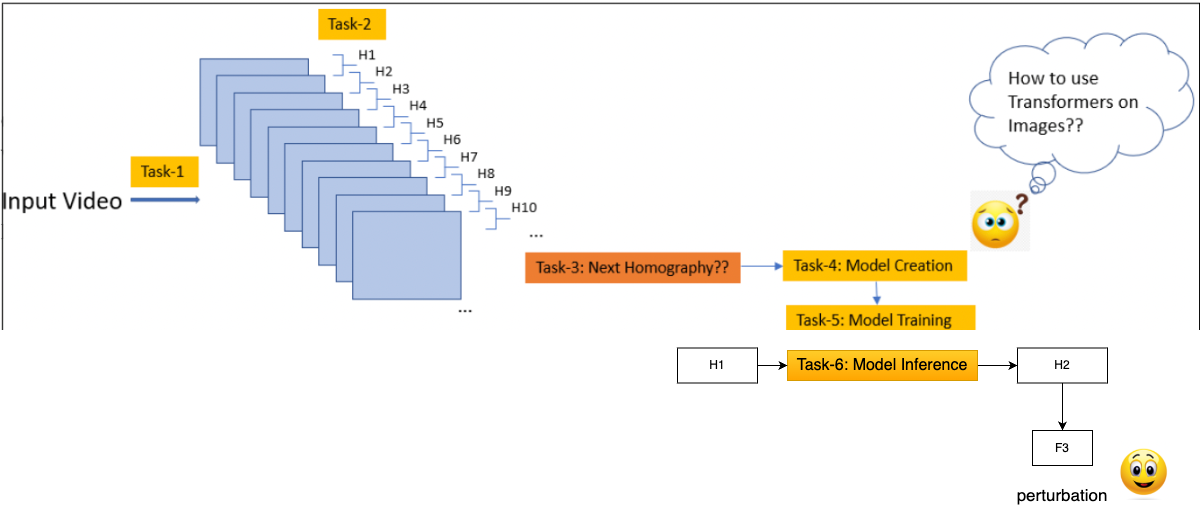
\includegraphics[scale=0.4]{img/novel.drawio.png}
    \caption{Overview of the methodology being used to generate a structured noise}
    \label{fig:Figure6}
\end{figure}

\section{REFERENCES}

[1] Zhang, Yifu, et al. "Bytetrack: Multi-object tracking by associating every detection box." European Conference on Computer Vision. Cham: Springer Nature Switzerland, 2022.

[2] Wang, Chien-Yao, Alexey Bochkovskiy, and Hong-Yuan Mark Liao. "YOLOv7: Trainable bag-of-freebies sets new state-of-the-art for real-time object detectors." Proceedings of the IEEE/CVF Conference on Computer Vision and Pattern Recognition. 2023.

[3] Deng, Jiankang, et al. "Retinaface: Single-stage dense face localisation in the wild." arXiv preprint arXiv:1905.00641 2019.

[4] Liang, Jingyun, et al. "SwinIR: Image restoration using swin transformer." Proceedings of the IEEE/CVF international conference on computer vision. 2021.

[5] Ledig, Christian, et al. "Photo-realistic single image super-resolution using a generative adversarial network." Proceedings of the IEEE conference on computer vision and pattern recognition. 2017.

[6] Deng, Jiankang, et al. "Arcface: Additive angular margin loss for deep face recognition." Proceedings of the IEEE/CVF conference on computer vision and pattern recognition. 2019.

[7] Goodfellow I. J., Shlens J., and Szegedy C. “Explaining and Harnessing Adversarial Examples”, ICLR, 2015.

[8] Kurakin A., Goodfellow I., and Bengio S. “Adversarial Examples in the Physical World”. ICLR 2017.

[9] N. Papernot, P. McDaniel, I. Goodfellow, S. Jha, Z.B. Celik, A. Swami, “Practical black-box attacks against machine learning”, in: Proceedings of the 2017 ACM on Asia conference on computer and communications security, 2017.

[10] Carlini N., Wagner D., “Towards evaluating the robustness of neural networks”, IEEE, 2017.

[11] Xiao, Chaowei, et al. "Generating adversarial examples with adversarial networks." arXiv preprint arXiv:1801.02610 (2018).

[12] Meden, Blaz et al. “Face deidentification with controllable Privacy protection”, Image and Vision Computing, 2023.

[13 ] Cao, Yuxin, et al. "Stylefool: Fooling video classification systems via style transfer." 2023 IEEE Symposium on Security and Privacy (SP). IEEE, 2023.
